\documentclass[
ngerman,
twoside,
pdfa=false,
ruledheaders=section,%Ebene bis zu der die Überschriften mit Linien abgetrennt werden, vgl. DEMO-TUDaPub
class=report,% Basisdokumentenklasse. Wählt die Korrespondierende KOMA-Script Klasse
thesis={type=sta},% Dokumententyp Thesis, für Dissertationen siehe die Demo-Datei DEMO-TUDaPhd
accentcolor=TUDa-2c,% Auswahl der Akzentfarbe
custommargins=false,% Ränder werden mithilfe von typearea automatisch berechnet
marginpar=false,% Kopfzeile und Fußzeile erstrecken sich nicht über die Randnotizspalte
%BCOR=5mm,%Bindekorrektur, falls notwendig
parskip=half-,%Absatzkennzeichnung durch Abstand vgl. KOMA-Sript
fontsize=11pt,%Basisschriftgröße laut Corporate Design ist mit 9pt häufig zu klein
%	logofile=tuda_logo.pdf, %Falls die Logo Dateien nicht installiert sind
]{tudapub}

%%%%%%%%%%%%%%%%%%%%%%%%%%%%
% Download des TU-Logos
%%%%%%%%%%%%%%%%%%%%%%%%%%%%
% https://download.hrz.tu-darmstadt.de/protected/CE/TUDa_LaTeX/tuda_logo.pdf
% Der Pfad zum Logo kann als "logofile" angegeben werden.

%%%%%%%%%%%%%%%%%%%
% Sprachanpassung & Verbesserte Trennregeln
%%%%%%%%%%%%%%%%%%%
\usepackage[english, main=ngerman]{babel}
\usepackage[autostyle]{csquotes}% Anführungszeichen vereinfacht
\usepackage{microtype}

%%%%%%%%%%%%%%%%%%%
% Literaturverzeichnis
%%%%%%%%%%%%%%%%%%%
\usepackage{biblatex}   % Literaturverzeichnis
\addbibresource{HausarbeitBib.bib}

%%%%%%%%%%%%%%%%%%%
% Paketvorschläge Tabellen
%%%%%%%%%%%%%%%%%%%
%\usepackage{array}     % Basispaket für Tabellenkonfiguration, wird von den folgenden automatisch geladen
\usepackage{tabularx}   % Tabellen, die sich automatisch der Breite anpassen
%\usepackage{longtable} % Mehrseitige Tabellen
%\usepackage{xltabular} % Mehrseitige Tabellen mit anpassarer Breite
\usepackage{booktabs}   % Verbesserte Möglichkeiten für Tabellenlayout über horizontale Linien

%%%%%%%%%%%%%%%%%%%
% Paketvorschläge Mathematik
%%%%%%%%%%%%%%%%%%%
\usepackage{mathtools} % erweiterte Fassung von amsmath
\usepackage{amssymb}   % erweiterter Zeichensatz
\usepackage[decimalsymbol=comma]{siunitx}   % Einheiten
\usepackage{amsmath}


%%%%%%%%%%%%%%%%%
% Eigenen Pakete Gruppe01
%%%%%%%%%%%%%%%%%%%%
%\usepackage[utf8]{inputenc}
%\usepackage[ngerman]{babel}
\usepackage{hyperref}
\usepackage{graphicx}
\usepackage{subcaption}
\usepackage{listings}
\usepackage[framed, numbered]{matlab-prettifier}
%\usepackage[style=numeric]{biblatex}
%\usepackage{amsthm}
%\usepackage[squaren]{SIunits}
\usepackage{enumitem}
\usepackage{tikz}
\usepackage{pgfplots}
\usepackage{pgfplotstable}
%\usepackage{booktabs}
\pgfplotsset{compat=1.12}
\usepackage{dsfont}

%%%%%%%%%%%%%%%%%%%
% verschiedene Nummerierung für Abbildungen und Formeln
%%%%%%%%%%%%%%%%%%%
\usepackage{chngcntr}
\counterwithout{equation}{chapter}


%%%%%%%%%%%%%%%%%%%
% Pseudocode
%%%%%%%%%%%%%%%%%%%
\usepackage[linesnumbered,lined,boxruled]{algorithm2e} % Package für Pseudocode

%%%%%%%%%%%%%%%%%%%
% Plotting und Grafik
%%%%%%%%%%%%%%%%%%%
\usepackage{tuda-pgfplots} % Package für Plotting with TUDa mods

%%%%%%%%%%%%%%%%%%%
% Sonstiges
%%%%%%%%%%%%%%%%%%%
\usepackage{blindtext} % Package für Blindtext

\begin{document}
	\title{Ausarbeitung Übung 5}
	%\subtitle{Ein Untertitel, wenn nötig}
	\author[D. Schiller, C. Kramer, S.Arnold, T. Lingenberg]{Dominik Schiller \and Constanze Kramer \and Simon Arnold \and Tobias Lingenberg} %optionales Argument ist die Signatur,
	%\reviewer{Gutachter 1 \and Gutachterin 2} %Gutachten
	
	%Diese Felder werden untereinander auf der Titelseite platziert.
	\department{} % Das Kürzel wird automatisch ersetzt und als Studienfach gewählt, siehe Liste der Kürzel im Dokument.

	
	\date{\today}
	%\examdate{\today}
	
	%	\tuprints{urn=1234,printid=12345}
	%	\dedication{Für alle, die \TeX{} nutzen.}
	
	\maketitle
	\pagenumbering{gobble} % Seitenzahlen angezeigt, startet ab dem Inhaltsverzeichnis
	
	
	%\affidavit
	%\AffidavitSignature
	%\AffidavitSignature
	
	
	%%%%%%%%%%%%%%%%%%%
	%Abstract / Kurzzusammenfassung
	%%%%%%%%%%%%%%%%%%%
	%\include{chapters/zusammenfassung}
	
	%%%%%%%%%%%%%%%%%%%
	%Inhaltsverzeichnis 
	%%%%%%%%%%%%%%%%%%%
	\cleardoublepage
	\tableofcontents % Erstellte ein Inhaltsverzeichnis
	
	%\cleardoublepage
	\pagenumbering{arabic} % Seitenzahlen angezeigt, startet ab dem Inhaltsverzeichnis
	\setcounter{page}{1} % Setzt den Seitenzahlenzähler auf 1
	
	%%%%%%%%%%%%%%%%%%%%%%%%%%%%%%%%%%%%%%%%%%%%%%%%%%%%%%%%%%%%%%%%%%%%%%%%%%%%%%%%%%%%%%%%%%%%%%%%%%
	
	% INHALT, am Besten ausgelagert in eigene Files/Kapitel und dann mit \include{Unterordner/Filename} eingefügt, sorgt für bessere Übersichtlichkeit und Fehlersuche. Einzelne Dateien sind aktuell im Ordner Sections abgelegt. 
	%%%%%%%%%%%%%%%%%%Einleitung%%%%%%%%%%%%%%%%%
	%\chapter{Einleitung}\label{sec:intro}
Diese Arbeit beschäftigt sich mit dem Übungsblatt 9 des Faches \glqq Einführung in die numerische Berechnung elektromagnetischer Felder\grqq{}.
Zunächst wird der primale Divergenz und Rotationsoperator in Octave implementiert und berechnet. Anschließend wird eine Materialmatrix berechnet. Abschließend wird das Magnetfeld von zwei stromdruchflossenen Leitern in Octave simuliert. 
	%%%%%%%%%%%%%%%%%%Haupteil%%%%%%%%%%%%%%%%%%%
	\chapter{Bearbeitung der Aufgaben}
\section{Geschichteter Plattenkondensator}

Um numerisch die Kapazität eines Plattenkondensators mit quer geschichteten Dielektrika, die eine linear steigende relative Permittivität aufweisen, zu bestimmen, kann man den linearen Verlauf über mehrere Schichten mit jeweils konstanter Permittivität approximieren. Wie bei numerischen Verfahren üblich wird die Approximation besser, je dünner die einzelnen Schichten gewählt werden.\\
\begin{figure}[h!]
	\centering
	\begin{subfigure}[h]{0.3\textwidth}
		\centering
		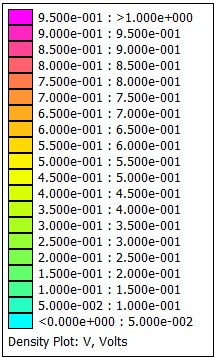
\includegraphics[width=\textwidth]{data/KondensatorN9_Legende}
		\caption{Skala}
		\label{fig:Skala1}
	\end{subfigure}
	\begin{subfigure}[h]{0.51\textwidth}
		\centering
		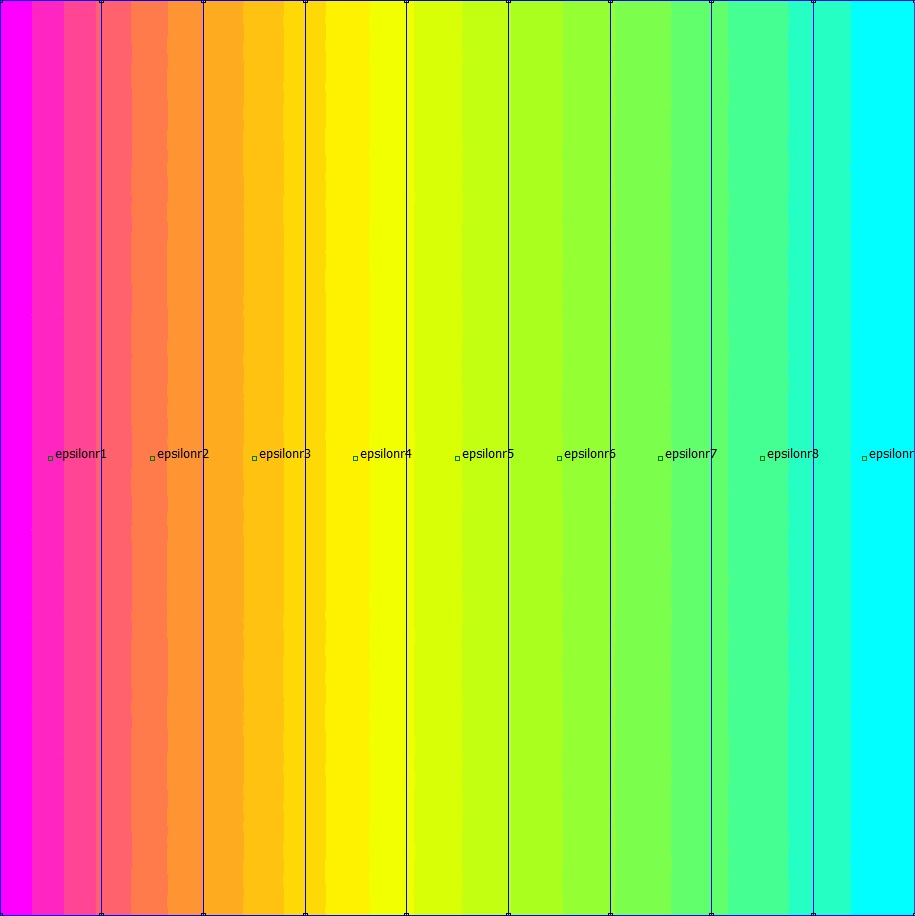
\includegraphics[width=\textwidth]{data/KondensatorN9}
		\caption{Potentialverlauf im Plattenkondensator mit 9 Schichten}
		\label{fig:N9}
	\end{subfigure}
	\caption{Potentialverlauf im Plattenkondensator mit 9 Schichten}
\end{figure} \\
Die Funktion \texttt{femmcapacity.m} bekommt als Parameter den Abstand $h$ zwischen den beiden Platten des Kondensators, die Kantenlänge $a$ der quadratischen Platten, $\varepsilon_{\mathrm{r,1}}$, $\varepsilon_{\mathrm{r,2}}$ und die Anzahl $N$ an Schichten übergeben. Mit Hilfe dieser Parameter wird daraus ein Plot für den Potentialverlauf im Kondensator erzeugt und die Kapazität der Anordnung berechnet. Die relative Permittivität variiert hierbei linear zwischen $\varepsilon_{\mathrm{r,1}} $ am linken Rand und $\varepsilon_{\mathrm{r,2}}$ am rechten Rand. Die zugehörigen Werte der relativen Permittivitäten der einzelnen Schichten $N_i$ lassen sich mit $$ \varepsilon_{\mathrm{r,i}} = \varepsilon_{\mathrm{r,1}} + \frac{i (\varepsilon_{\mathrm{r,2}}-\varepsilon_{\mathrm{r,1}})}{N-1}$$ berechnen. Im Folgenden wird der Abstand zwischen den Platten und die Kantenlänge mit \SI{30}{\centi\meter} angenommen. Wählt man 9 Schichten, $\varepsilon_{\mathrm{r,1}} = 1$ und $\varepsilon_{\mathrm{r,2}} = 2$  erhält man den in Abbildung \ref{fig:N9} zu sehenden Potentialverlauf und eine Kapazität $ C_1 = \SI{3,793}{\pico\farad}$.\\ \\
Wiederholt man die Simulation für $N = 1,2,3,...,20$ Schichten und lässt sich in einem Konvergenz-Plot (Abbildung \ref{fig:semilogy}) die Kapazität in Abhängigkeit der Schichtanzahl anzeigen, wird deutlich, dass schon nach $N=3$ Schichten die Kapazität annähernd exakt bestimmt wird und weitere Verfeinerungen nur noch marginale Verbesserungen der Approximation erzielen. \\ \\

\begin{figure}[tpbh]
	\centering
	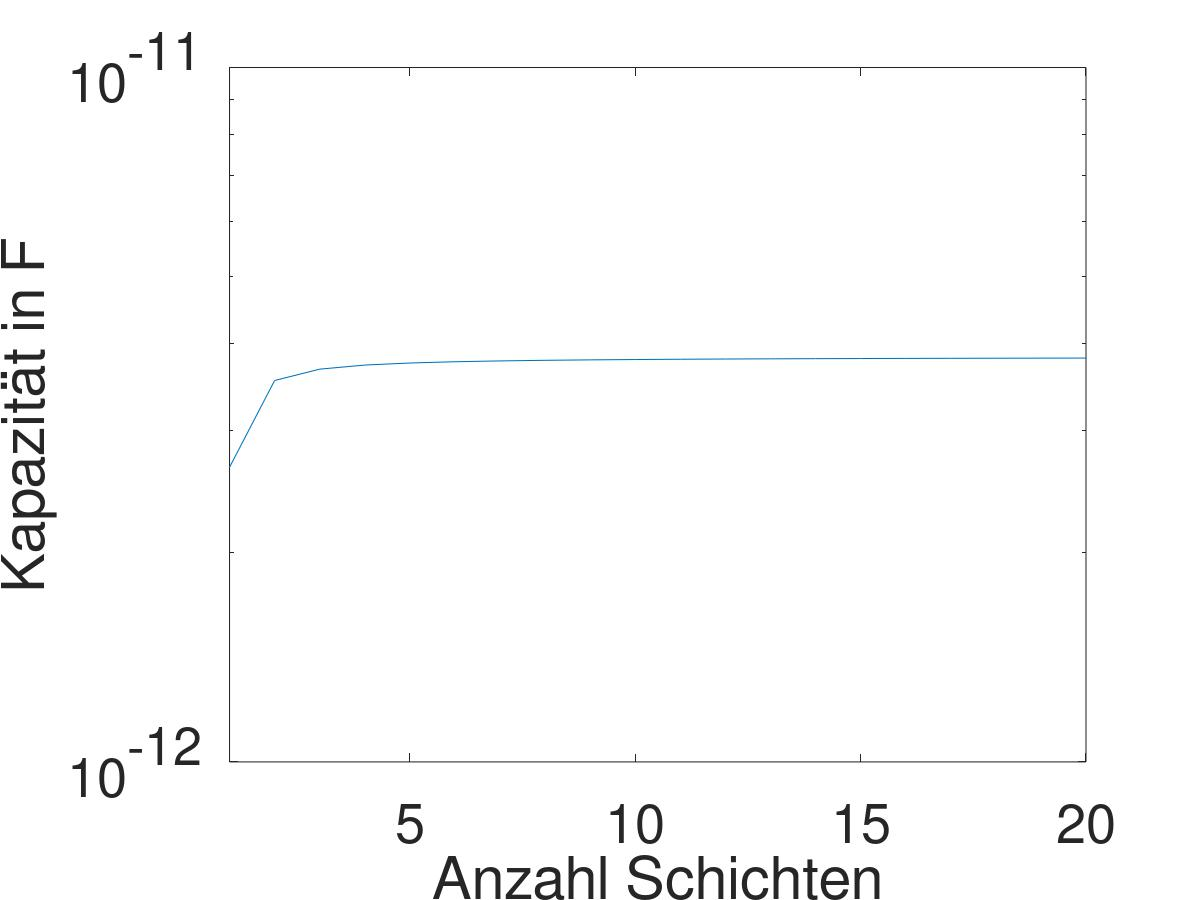
\includegraphics[width=.8\textwidth]{data/Kapazitaet}
	\caption{Änderung der Kapazität mit steigender Anzahl an Schichten im Plattenkondensator}
	\label{fig:semilogy}
\end{figure}


Die Option \texttt{'Vector Plot'} in FEMM ist nützlich, um den Verlauf des elektrischen Feldes besser darzustellen. Die Richtung der Pfeile zeigt an in welche Richtung das Feld an dieser Stelle zeigt und die Länge der Pfeile deutet die Stärke an dieser Stelle an.
\newpage
In Abbildung \ref{fig:N1_EFeld} sieht man den Plot für den homogenen Plattenkondensator und in Abbildung \ref{fig:N9_EFeld} für den geschichteten Fall. Vergleicht man beide Abbildungen fällt auf, dass das elektrische Feld im homogenen Plattenkondensator homogen verteilt ist. Beim geschichteten Plattenkondensator hingegen ist das elektrische Feld deutlich stärker auf der Seite mit der geringeren relativen Permittivität und nimmt immer weiter ab, je höher die relative Permittivität ist.

\begin{figure}[h]
	\begin{subfigure}[c]{0.2\textwidth}
		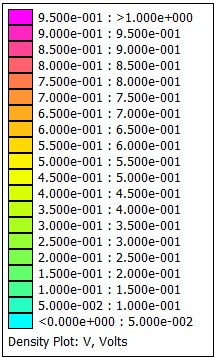
\includegraphics[width=\textwidth]{data/KondensatorN9_Legende}
		\caption{Skala}
		\label{fig:Skala2}
	\end{subfigure}
	\begin{subfigure}[c]{0.35\textwidth}
		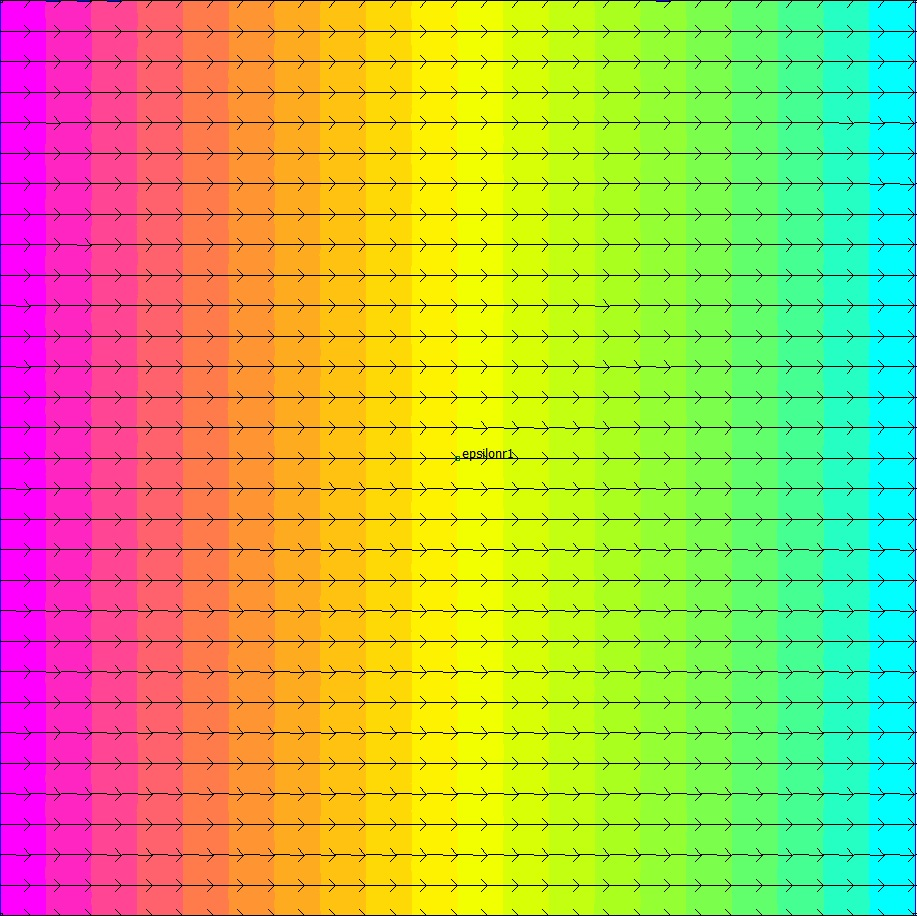
\includegraphics[width=\textwidth]{data/KondensatorN1_EFeld}
		\caption{Potentialverlauf und elektrische Feldstärke im homogenen Plattenkondensator}
		\label{fig:N1_EFeld}
	\end{subfigure}
	\begin{subfigure}[c]{0.35\textwidth}
		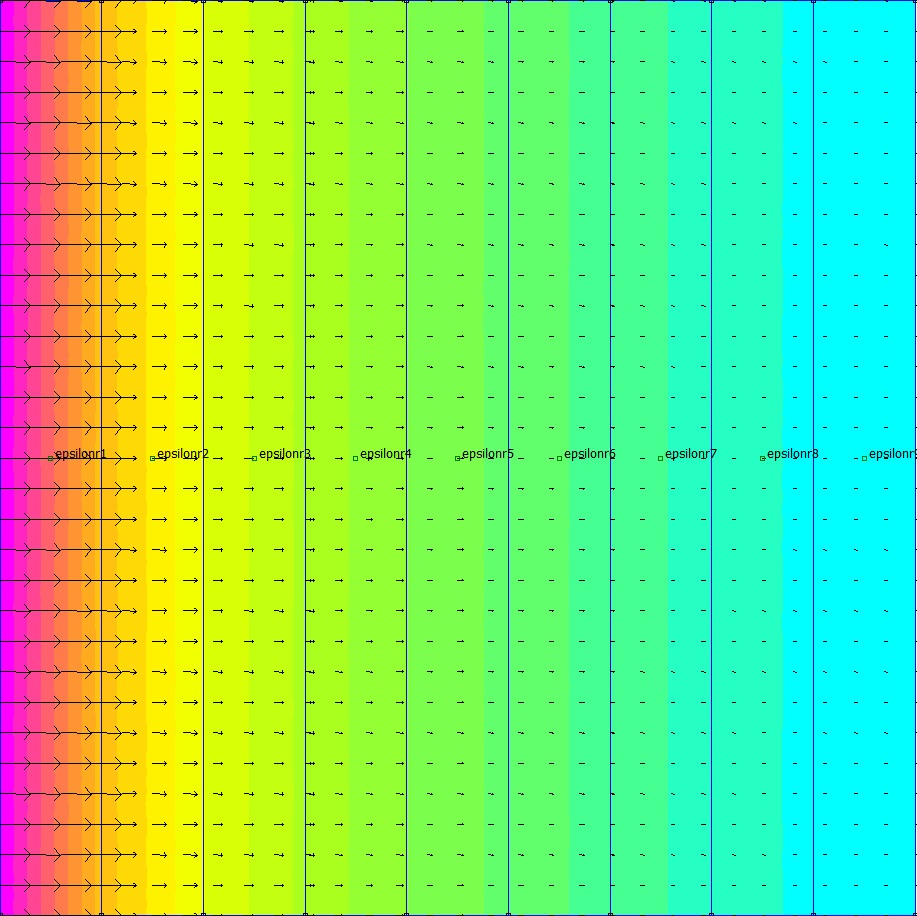
\includegraphics[width=\textwidth]{data/KondensatorN9_EFeld}
		\caption{Potentialverlauf und elektrische Feldstärke im Plattenkondensator mit 9 Schichten}
		\label{fig:N9_EFeld}
\end{subfigure}
	\caption{Potentialverlauf und elektrische Feldstärke im homogenen und im geschichteten Plattenkondensator}
\end{figure}

Bestimmt man die Kapazität für $\varepsilon_{\mathrm{r,1}} = 1$ und $\varepsilon_{\mathrm{r,2}} = 10$ und $N = 9$ und vergleicht diese mit der vorher bestimmten Kapazität $C_1$ stellt man fest, dass durch eine höhere relative Permittivität auch die Kapazität von $\SI{3,793}{\pico\farad}$ auf $\SI{8,916}{\pico\farad}$ steigt.


	\section{Aufgabe 5.3}
Wie in der vorherigen Aufgabe und den bisherigen Ausarbeitungen gezeigt, lassen sich mit Hilfe von FEMM sehr gute Simulationen von Plattenkondensatoren erzeugen. Aber auch Kugelkondensatoren lassen sich mit FEMM simulieren und berechnen. \\
Die Methode \texttt{spherecapacity.m}, die im Anhang zu finden ist, nimmt die zwei Parameter $R_1$, der den Innenradius beschreibt und $\varepsilon_r$, das die relative Permittivität des Dielektrikums darstellt, entgegen. Aus der Aufgabenstellung geht hervor, dass für den zweiten zur Berechnung der Kapazität benötigten, Parameter $R_2 = R_1 + \SI{7}{\centi\meter}$ gilt. $R_2$ ist der Außenradius des Kugelkondensators. Optional könnte man die Methode auch so schreiben, dass $R_2$ übergeben werden kann.\\
Im Vergleich zu den bisherigen Simulationen in FEMM haben wir nun kein planares Problem mehr, sondern ein achsensymmetrisches. In der Problemdefinition in Zeile 6 wird deshalb ein \texttt{'axi'} übergeben. Damit wird bestimmt, dass sich die erzeugte Fläche in Abbildung \ref{fig:KK} nicht in die Tiefe entwickelt, sondern um die z-Achse gedreht wird. Dadurch erhalten man eine 3-Dimensionale Kugel, die FEMM zwar nicht darstellen, aber berechnen kann.\\ \\
In den Zeilen 12 bis 26 werden zwei Halbkreise erzeugt, der innere Halbkreis wird auf \SI{1}{\volt} geladen, am äußeren Halbkreis liegt eine Spannung von \SI{0}{\volt} an. Des Weiteren werden zwischen Zeile 28 und 31 zwei Blocklabel erstellt, das erste Label liegt zwischen den beiden Halbkreisen und beinhalten die Informationen über die relative Permittivität des Dielektrikums. Mit dem zweiten Label wird sichergestellt, dass nur die von den beiden Halbkreisen und deren Verbindungslinien eingeschlossene Fläche zur Simulation genutzt wird. Hierzu wird dem Label die Property \texttt{<No Mesh>} übergeben. Schließlich werden in Zeile 38 und 39 die Verbindungslinien zwischen den Halbkreisen erstellt, um eine abgeschlossene Fläche zu erzeugen. \\ \\
\begin{figure}[h]
	\centering
	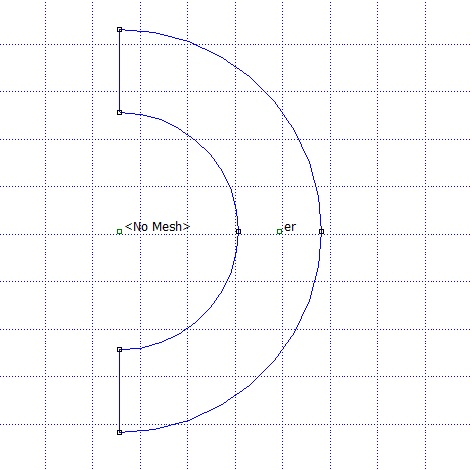
\includegraphics[width=.45\textwidth]{data/Kugelkondensator}
	\caption{Ein mit Hilfe der Routine \texttt{spherecapacity} erzeugter Kugelkondensator mit $R_1 = \SI{7}{\centi\meter}$ }
	\label{fig:KK}
\end{figure}

Mit 
\begin{equation}
	C = 4\pi\varepsilon_0\varepsilon_r\frac{R_2R_1}{R_2-R_1}
	\label{eq:Kapa}	
\end{equation}
lässt sich die Kapazität eines homogenen Kugelkondensators berechnen.
Um den Einfluss der Radien auf die Kapazität zu untersuchen, wurden der Methode \texttt{spherecapacity.m} 100 verschiedene Radien $R_1 \in \mathbb{N}, R_1 \in [1,100]$, mit der Einheit \si{\centi\meter} übergeben. Für den Radius $R_2$ gilt weiterhin
\begin{equation}
	R_2 = R_1 + \SI{7}{\centi\meter}.
	\label{eq:R2}
\end{equation}
Die berechneten Kapazitätswerte sind in Abbildung \ref{fig:Kapa} graphisch dargestellt. Die Formel 
\begin{equation}
	C = 4\pi\varepsilon_0\varepsilon_r\frac{(R_1+\SI{0.07}{\meter})R_1}{R_1+\SI{0.07}{\meter-R_1}}
\end{equation}
ergibt sich indem man (\ref{eq:R2}) in (\ref{eq:Kapa}) einsetzt. Durch weiteres vereinfachen folgt, dass die Kapazität
\begin{equation}
	C = 4\pi\varepsilon_0\varepsilon_r\frac{R_1^2+\SI{0.07}{\meter}}{(\SI{0.07}{\meter)}}
\end{equation}
quadratisch von $R_1$ abhängt, daraus ergibt sich ein quadratischer Verlauf der Kapazität des Kugelkondensators mit steigendem Innenradius.

\begin{figure}
	\centering
	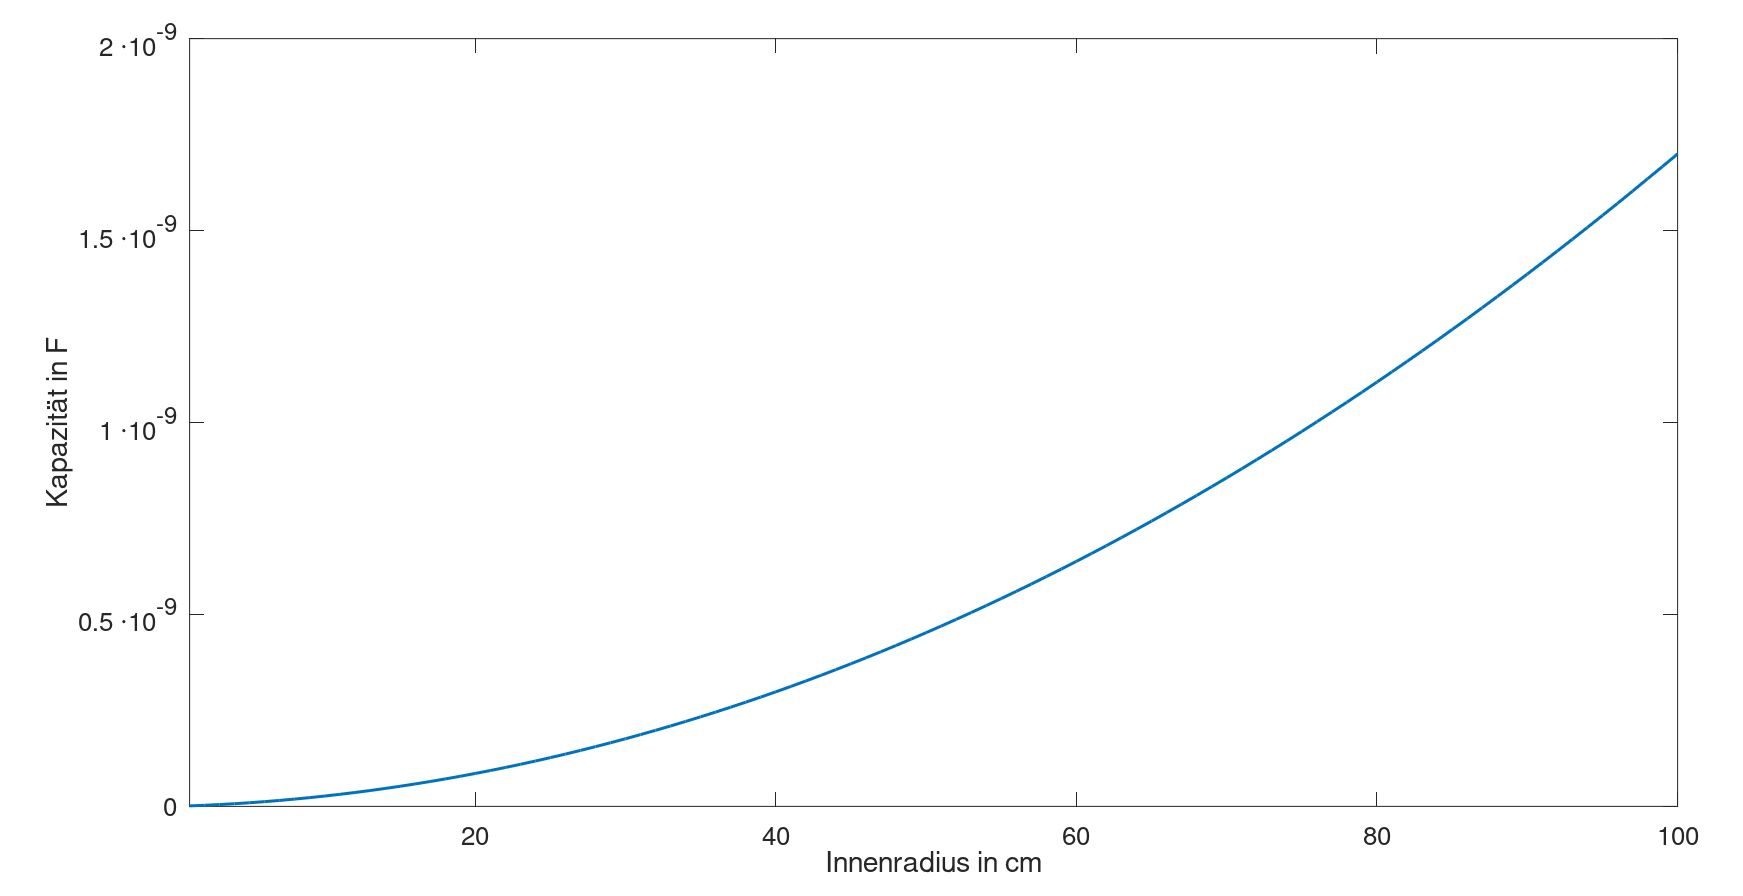
\includegraphics[width=\textwidth]{data/Kugelkapa}
	\caption{Entwicklung der Kapazität mit steigendem Radius $R_1 \in \mathbb{N}, R_1 \in [1,100]$ und $R_2 = R_1 + \SI{7}{\centi\meter}$}
	\label{fig:Kapa}
\end{figure}
	%\section{Numerische Lösung linearer Gleichungssysteme}
Bei numerischen Berechnungen spielen lineare Gleichungssysteme der Form \textbf{Ax}=\textbf{y} oft eine überaus wichtige Rolle. Daher ist es sinnvoll und von Nöten effiziente Lösungsverfahren für diese Gleichungssysteme zu entwickeln und anzuwenden. In diesem Abschnitt werden verschiedene Verfahren in Octave implementiert und an beispielhaften Gleichungssystemen getestet und gegeneinander verglichen.\\ \\
Zunächst wird eine vorgegebene quadratische Matrix betrachtet. Mit Hilfe des Befehls \texttt{spy} lassen sich Matrizen in Octave graphisch darstellen. In Abb. \ref{fig:bspMat} ist diese Graphik zu sehen, die blauen Punkte in dem Plot sind Einträge, die ungleich null sind. Zählt man diese mit dem Befehl \texttt{nnz} findet man heraus, dass 3678 der 158404 Einträge ungleich null sind. Weiterhin lässt sich aus der Abbildung und der Darstellung der Werte in Octave herausfinden, dass es sich um eine symmetrische Matrix handelt, das heißt die Einträge der Matrix sind spiegelsymmetrisch bezüglich der Hauptdiagonalen. \\ \\
\begin{figure}[h]
	\begin{subfigure}[c]{.48\textwidth}
		\centering
		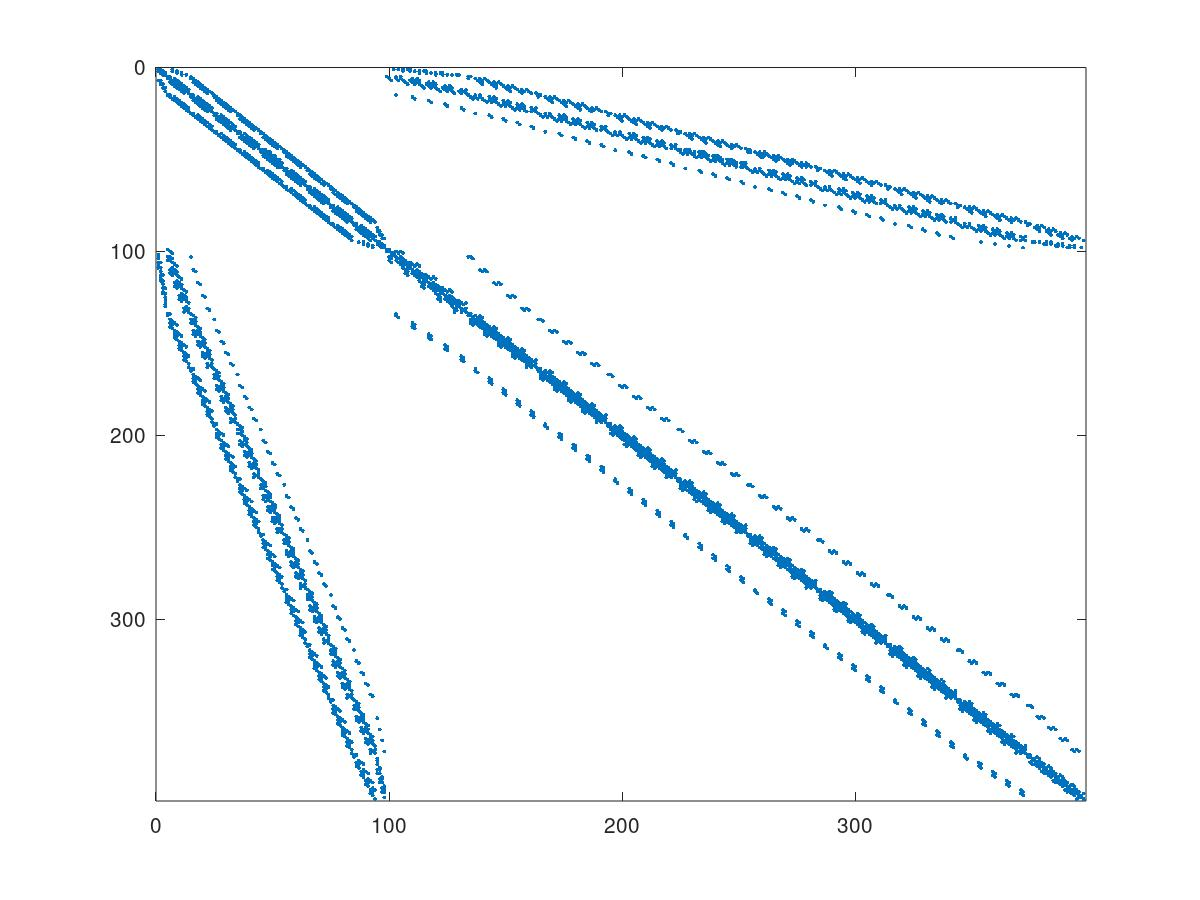
\includegraphics[width=\textwidth]{data/MatrixBsp}
		\subcaption{Graphische Darstellung der mit Octave eingelesene Beispielmatrix}
		\label{fig:bspMat}
	\end{subfigure}
	\begin{subfigure}[c]{.48\textwidth}
		\centering
		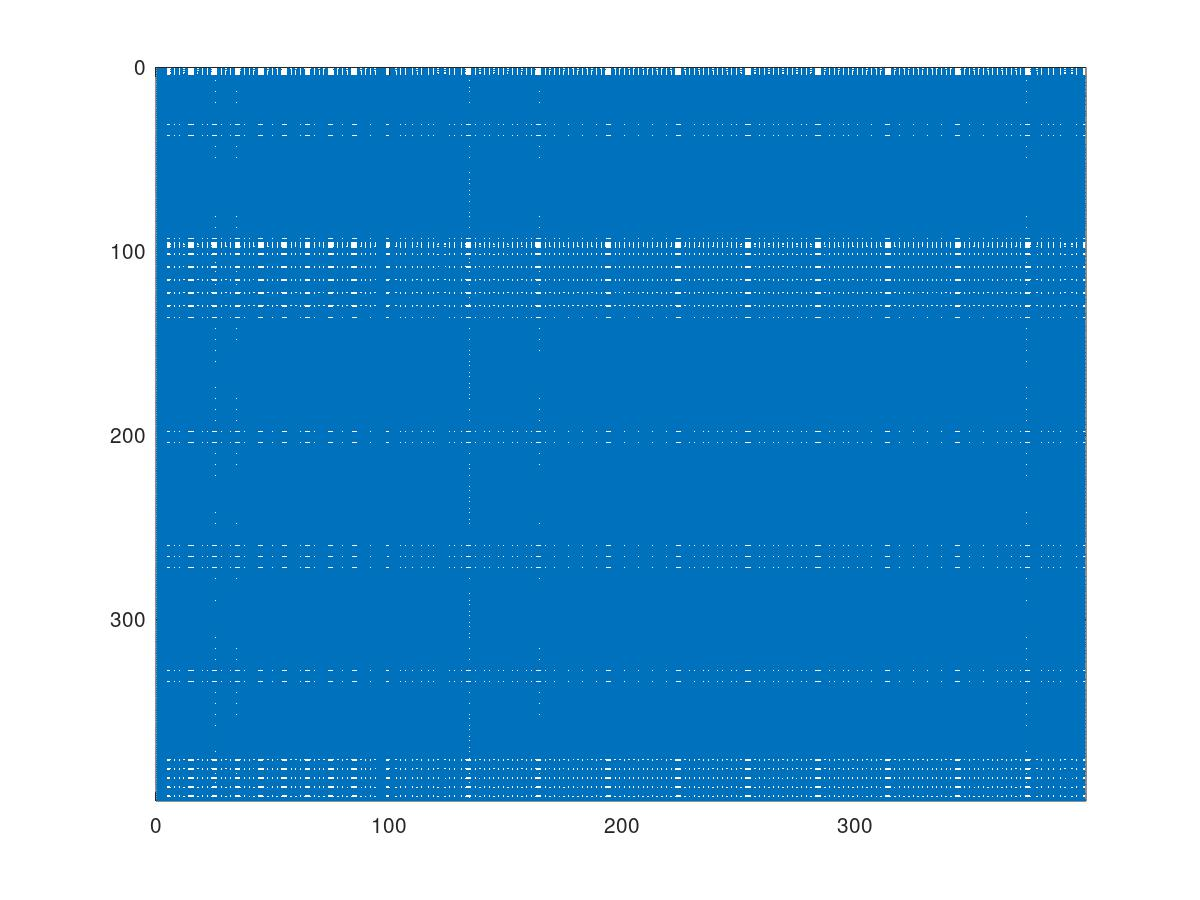
\includegraphics[width=\textwidth]{data/MatrixInv}
		\subcaption{Berechnete Inverse der eingelesenen Matrix}
		\label{fig:inv}\vspace{12pt}
	\end{subfigure}
	\caption{Graphische Darstellung von Matrizen, die blauen Punkte stellen Einträge dar, die ungleich null sind}
\end{figure} \\ 
Nun soll ein erstes Lösungsverfahren in Octave implementiert werden. Das \textsc{Gauss
'sche}-Eliminationsverfahren wurde in Listing \ref{lst:Elim} implementiert. Die Routine \texttt{gaussElim} erhält einen stehenden Vektor \textbf{b} mit Länge $n$ und eine quadratische Matrix \textbf{A} der Größe $n \times n$. Die Rückgabe ist ein Vektor \textbf{x} mit Länge $n$, der die berechneten Lösungen $x_{1}, \dots, x_{n}$ unseres linearen Gleichungssystems enthält.\\ \\
Zunächst wird \texttt{n}, also die Größe der Matrix bestimmt, daraufhin wird der Ergebnisvektor \textbf{x} mit entsprechender Länge erzeugt. In Zeile 4 und 5 werden zwei Laufvariablen initialisiert, \texttt{j} läuft hierbei über die Spalten, \texttt{i} über die Zeilen. Das Ziel des Algorithmus ist es schrittweise aus der übergebenen Matrix eine untere Dreiecksmatrix zu erstellen. Hierzu werden sogenannte Eliminationsfaktoren bestimmt, siehe Listing \ref{lst:Elim} Zeile 6. Mit Hilfe einer weiteren Laufvariable \texttt{k}, die über die Spalten von \texttt{j} bis \texttt{n} läuft. In der Schleife, Zeile 7 bis 9, werden Zeilenadditionen durchgeführt, um so Spalte für Spalte Nulleinträge zu erzeugen. Auch der Vektor \textbf{b} wird entsprechend angepasst. \\
In den Zeilen 14 bis 17 wird das Gleichungssystem final gelöst, die einzelnen $x_{1}, \dots, x_{n}$ werden von unten nach oben mit Hilfe der Matrix und dem Vektor \textbf{b} berechnet.  \\
Durch die drei ineinander geschachtelten For-Schleifen in den Zeilen 4 bis 12 erhalten wir eine kubische Anzahl an Rechenschritten, $n^{3}-n^{2}$, Zeile 14 bis 17 führen zu einem zusätzlichen Rechenaufwand von $n^{2}-n$, daraus ergibt sich die Abschätzung $\mathcal{O}(n^{3})$.
\lstinputlisting[label=lst:Elim,numbers=left]{data/gaussElim.m} 
Lineare Gleichungssysteme lassen sich auch mit Hilfe der Inversen einer Matrix bestimmen. In Octave geht dies mit dem Befehl \texttt{inv(A)}. Wie aus Abbildung \ref{fig:inv}, verglichen mit Abbildung \ref{fig:bspMat}, hervorgeht, hat die Invertierte Matrix deutlich mehr Einträge, die ungleich null sind. Die Berechnung der Inversen benötigt sehr viel Arbeitsspeicher und es werden deutlich mehr Rechenoperationen ausgeführt, um die Lösungen zu berechnen.\\ \\

%%%%%%%%%%%%%%%%%%%%%%%%% Aufgabenteil d %%%%%%%%%%%%%%%%%%%%%%%%%%%%
Eine weitere Methode mit der lineare Gleichungssysteme effizient berechnet werden können ist die LUPQ-Zerlegung. Bei der LUPQ-Zerlegung wird die Matrix \textbf{A} mit Hilfe des bereits vorgestellten \textsc{Gauss'schen}-Eliminationsverfahren in eine obere und eine untere Dreiecksmatrizen aufgeteilt, es gilt $\textbf{A} = \textbf{L} \textbf{U}$. Mit Hilfe von Vorwärts-/Rückwärtseinsetzen lässt sich nun das Gleichungssystem lösen. Zum Lösen wird zunächst vorwärts $$ \textbf{Ly} = \textbf{b}$$ eingesetzt und anschließend rückwärts $$ \textbf{Ux} = \textbf{y}$$ berechnet. Zum berechnen unterschiedlicher Seiten \textbf{b} muss die Matrix nicht neu zerlegt, sondern nur das Vorwärts-/Rückwärtseinsetzen betrachtet werden. Auch dieses Verfahren ist in Octave bereits vorimplementiert und lässt sich mit dem Befehl \texttt{lu(A)} aufrufen. Es ergeben sich bei dieser Methode Unterschiede, die durch die Anzahl der zur Verfügung gestellten Variable in denen die Lösung gespeichert werden soll, hervorgerufen werden.\\
Gibt man der Methode zwei Variablen zum Speichern der Ergebnisse vor, so entsteht nicht wie erwartet eine obere und eine untere Dreiecksmatrix, sondern die in Abbildung \ref{fig:LLU} zu sehende Matrix \textbf{L} und die in Abb. \ref{fig:ULU} Matrix \textbf{U}. Stellt man der Routine vier Variablen \texttt{[L, U, P, Q]} zum Speichern zur Verfügung so entsteht wie in Abb. \ref{fig:LLUPQ} und \ref{fig:ULUPQ} zu sehen ist jeweils eine obere und untere Dreiecks Matrix. Zudem haben diese Matrizen deutlich weniger Einträge. \textbf{P} ist eine Permutationsmatrix. Mit dieser werden Zeilen und Spalten der Ausgangsmatrix \textbf{A} vertauscht, um zu kleine Pivot Elemente, die zu großen Rundungsfehlern führen können, zu verhindern und zu garantieren, dass die Zerlegung in eine obere und untere Dreiecksmatrix möglich ist. 

\begin{figure}[h!]
	\begin{subfigure}[h]{.48\textwidth}
		\centering
		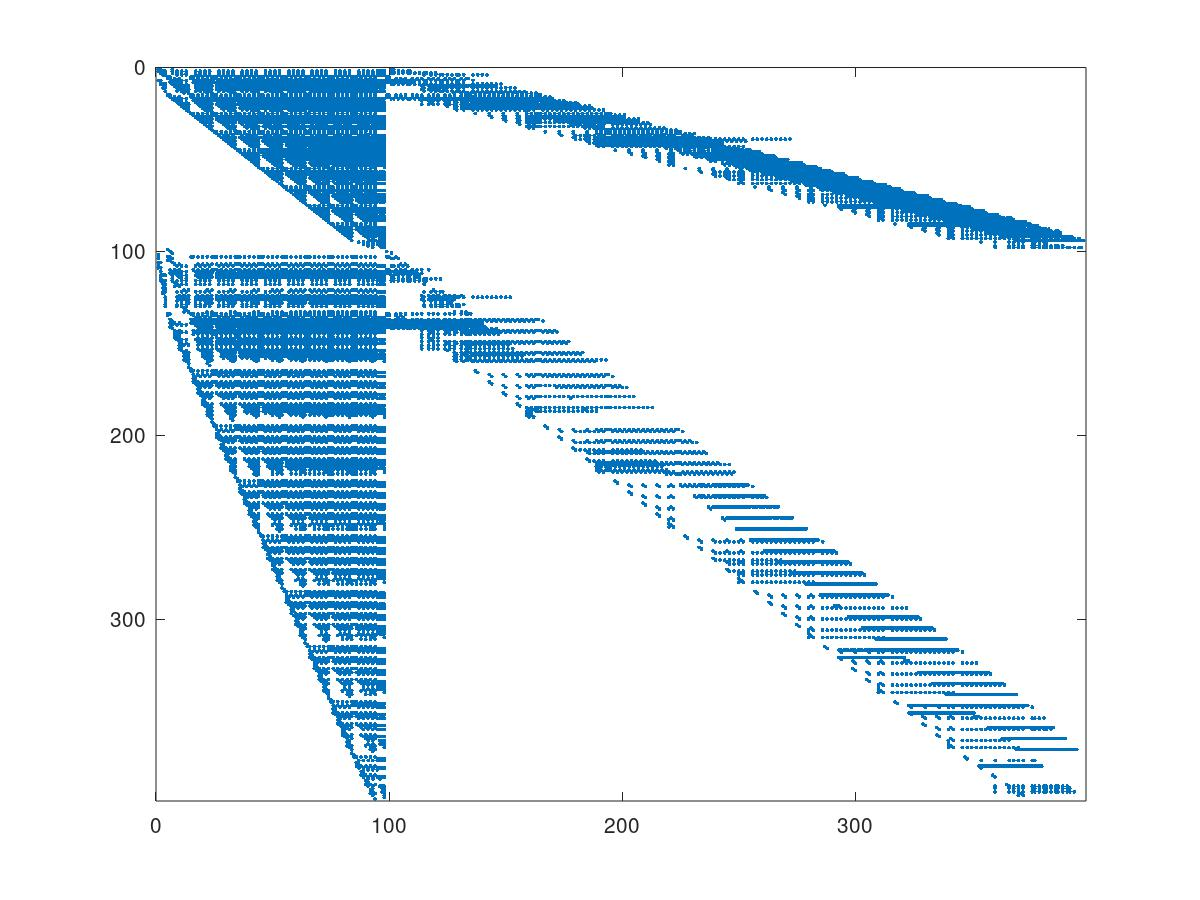
\includegraphics[width=\textwidth]{data/LLU}
		\subcaption{Matrix \textbf{L} nach LU-Zerlegung}
		\label{fig:LLU}
	\end{subfigure}
	\begin{subfigure}[h]{.48\textwidth}
		\centering
		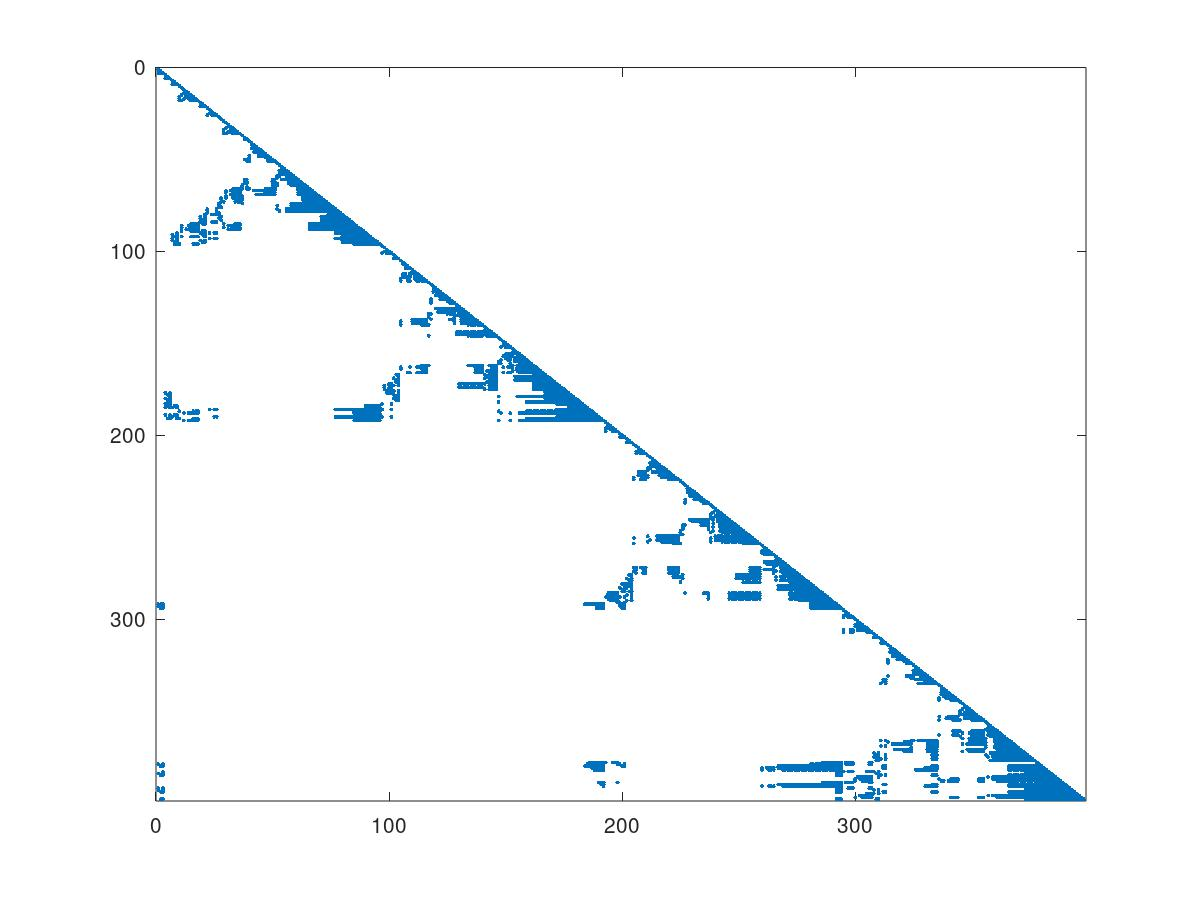
\includegraphics[width=\textwidth]{data/LLUPQ}
		\subcaption{Matrix \textbf{L} nach LUPQ-Zerlegung}
		\label{fig:LLUPQ}
	\end{subfigure}
	\begin{subfigure}[h]{.48\textwidth}
		\centering
		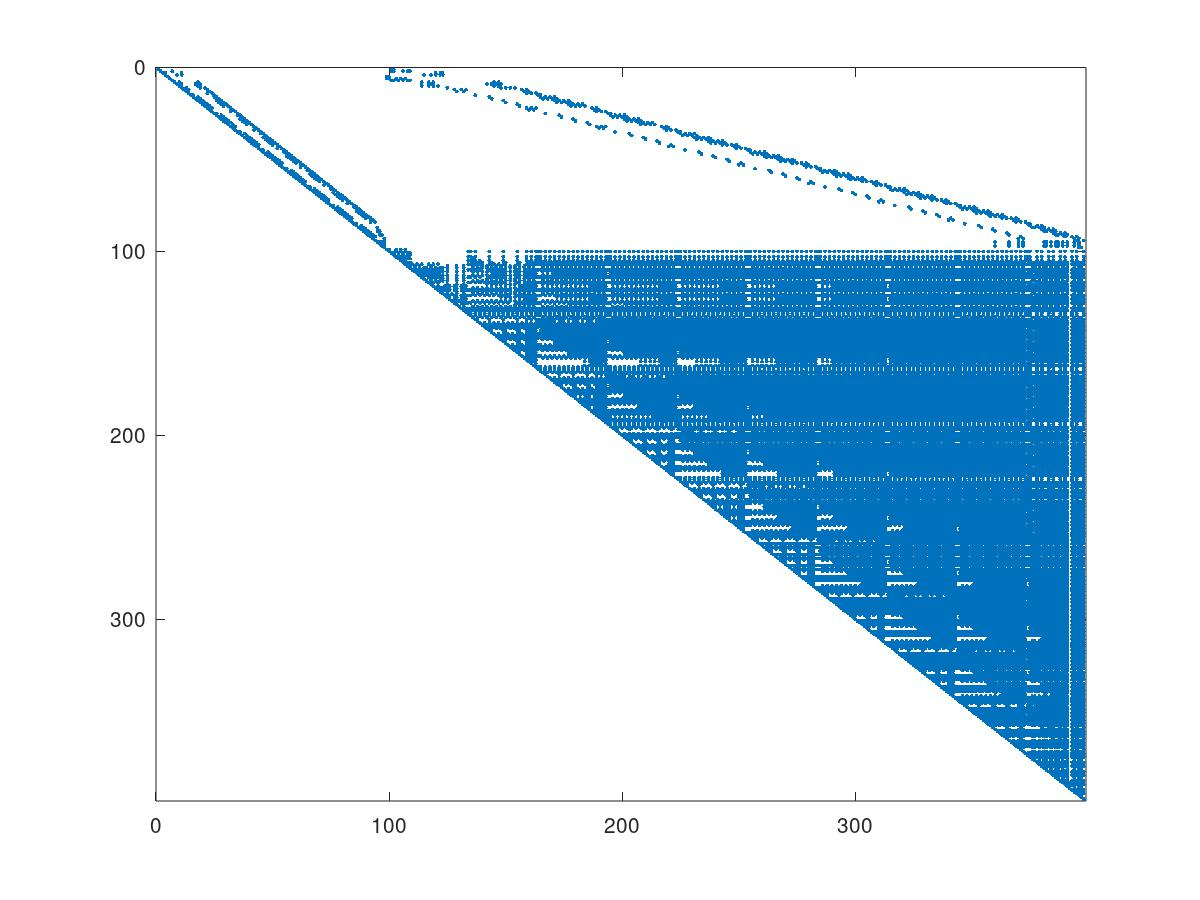
\includegraphics[width=\textwidth]{data/ULU}
		\subcaption{Matrix \textbf{U} nach LU-Zerlegung}
		\label{fig:ULU}
	\end{subfigure}
	\begin{subfigure}[h]{.48\textwidth}
		\centering
		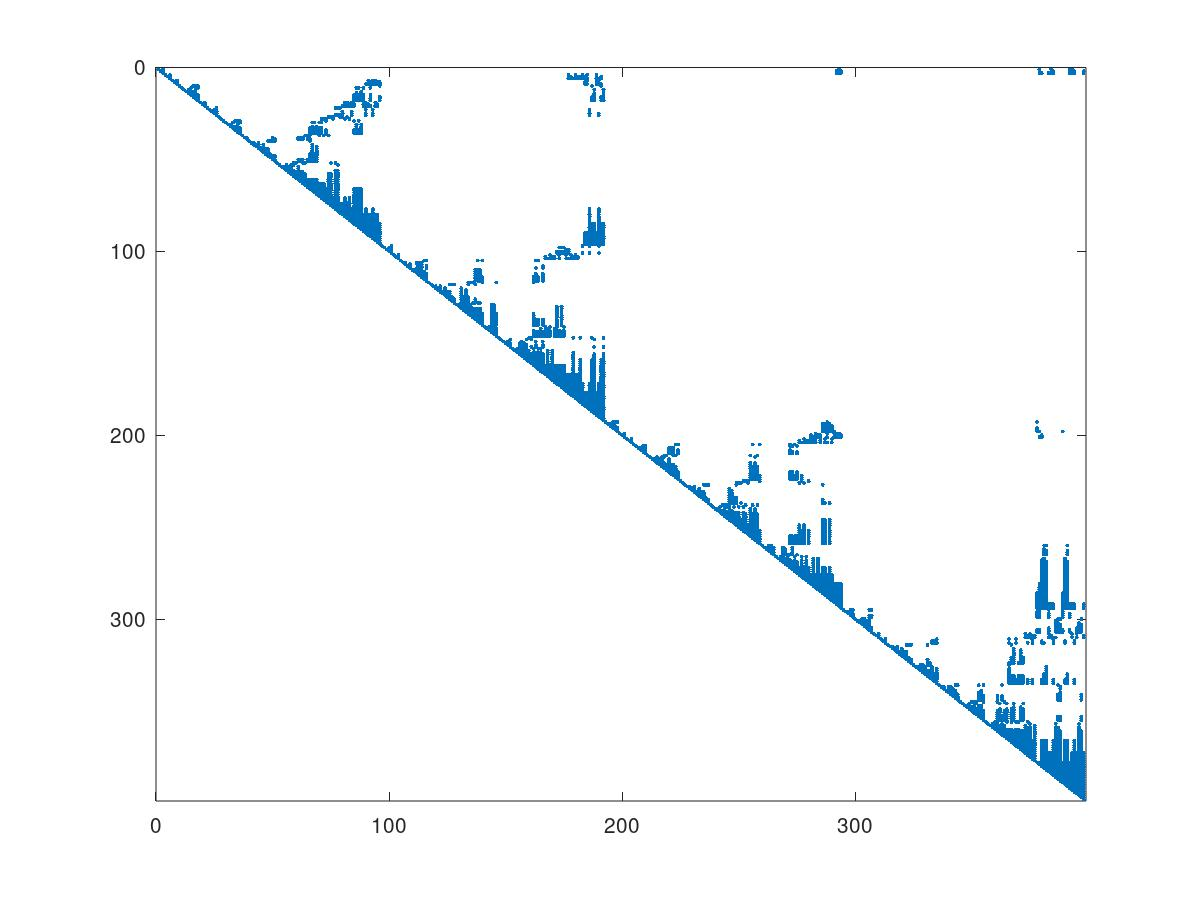
\includegraphics[width=\textwidth,]{data/ULUPQ}
		\subcaption{Matrix \textbf{U} nach LUPQ-Zerlegung}
		\label{fig:ULUPQ}
	\end{subfigure}\hspace{40pt}
\caption{Darstellung der unterschiedlichen Matrizen, die abhängig der zur Verfügung gestellten Lösungsvariablen entstehen}
\end{figure}
Um den zeitlichen Aufwand der einzelnen Lösungsverfahren besser vergleichen zu können wird im Folgenden eine Messung der benötigten Rechenzeit in Octave durchgeführt und beschrieben. Die zu vergleichenden Lösungsverfahren zur Berechnung linearer Gleichungssysteme sind die LUPQ-Zerlegung, Lösung mit Hilfe des Backslash-Operators und die Berechnung mit der Inversen.\\ \\
Verschiedene tridiagonale Testmatrizen \textbf{A} der Größe $n \times n$ mit $n \in [500, 1000, 2000, 4000, 8000]$ haben jeweils 10 unterschiedliche, zufällige Seiten \textbf{b} zugewiesen bekommen. Die Zeit zur Berechnung jeder einzelnen Seite wurde gespeichert, die Berechnung der Inversen bzw. der LUPQ Zerlegung fließt nur bei der ersten Berechnung mit in die Rechenzeit ein. \\
Die Rechenzeit, die benötigt wurde um alle 10 Seiten zu berechnen wurde schließlich durch 10 geteilt, um eine durchschnittliche Rechenzeit zu erhalten. Die Ergebnisse wurden abschließend auf einem doppelt logarithmischen Koordinatensystem geplottet, wobei die x-Achse die Größe $n$ der Matrix ist und die y-Achse die zur Berechnung einer Seite benötigte Rechenzeit.
\begin{figure}
	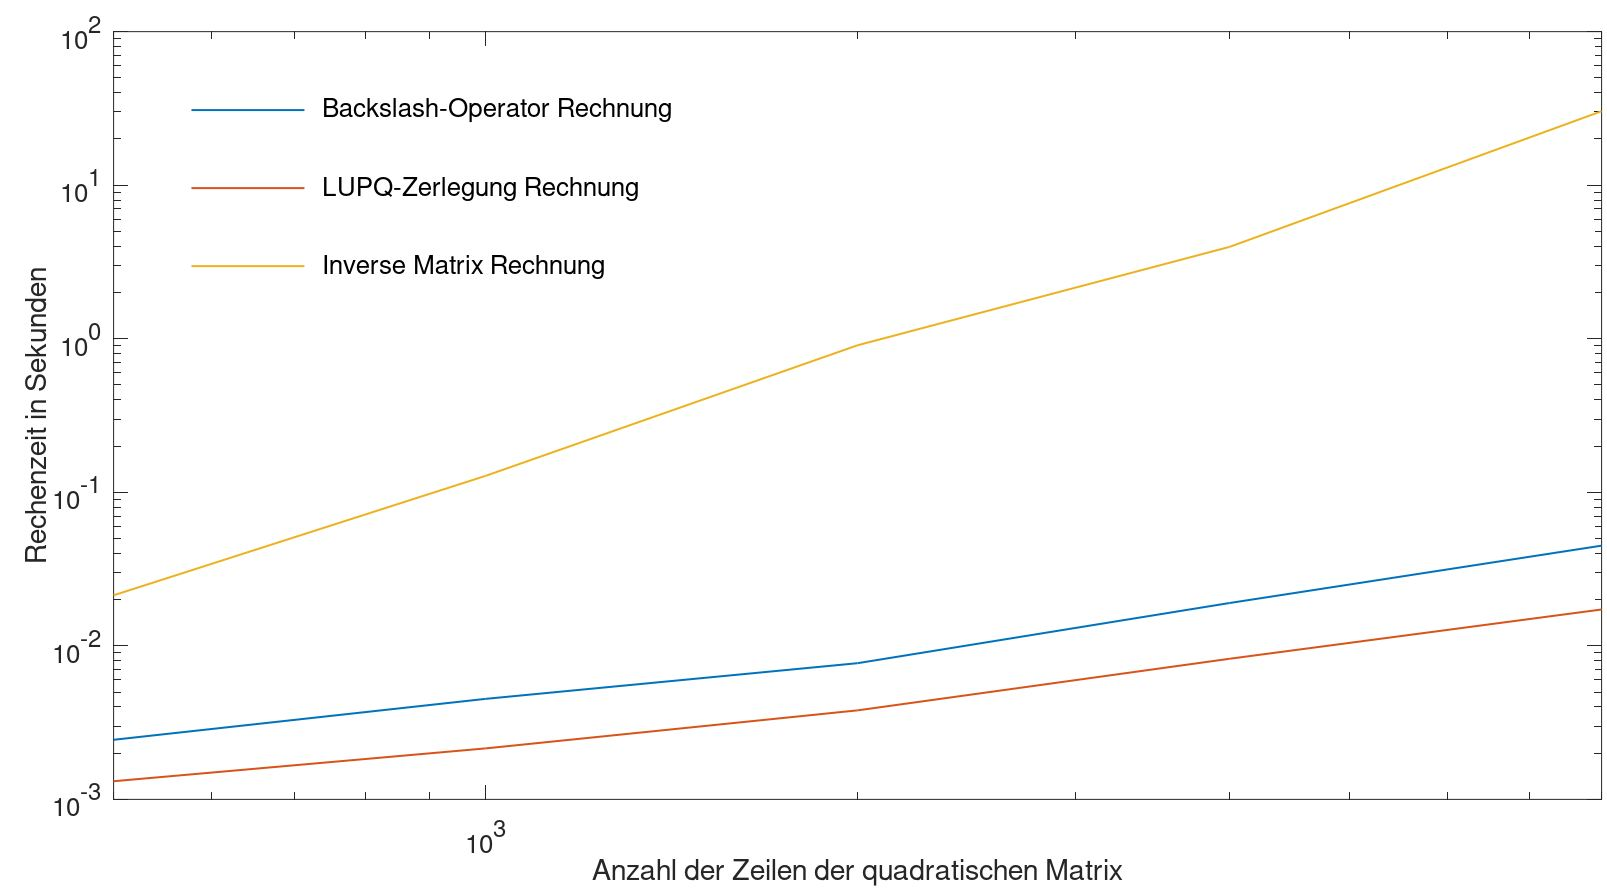
\includegraphics[width=\textwidth]{data/LaufzeitPlot}
	\caption{Graphische Darstellung der Rechenzeit, die unterschiedliche Lösungsverfahren zum Lösen linearer Gleichungen benötigen}
	\label{fig:Laufzeit}
\end{figure}
\\ \\
Wie aus Abbildung \ref{fig:Laufzeit} erkenntlich ist, benötigt die LUPQ-Zerlegung die geringste Zeit, um die Gleichungssysteme zu lösen. Der Backslash Operator benötigt mehr Zeit, ist aber, verglichen zur Berechnung mit Hilfe der Inversen, immer noch effizient. 
	
	%%%%%%%%%%%%%%%%%%Fazit%%%%%%%%%%%%%%%%%%%%%%
	%\chapter{Fazit}\label{sec:fazit}
%\addcontentsline{toc}{section}{Fazit}
Die erste Aufgabe ergab, dass sich die beiden Leiter des Koaxialkabels wie die Platten eines Plattenkondensators verhalten. Darüber hinaus ergibt sich, dass man durch Anfügen von weiteren Segmenten an die Schaltung eine Verkleinerung der Schwingfrequenz bewirkt.
Differentialgleichungen können häufig, wie sich in Aufgabe zwei zeigt, leichter im Frequenzbereich als im Zeitbereich gelöst werden. Die durch Lösen der Differentialgleichung analytisch berechneten Ergebnisse für Zeit- und Frequenzverhalten stimmen dabei mit der numerischen Simulation durch LTSpice überein.
Die Ergebnisse der dritten Aufgabe ergeben, dass sich die Feldlinien eines Kondensators in einem Simulationskäfig nicht nur senkrecht zu den Platten bewegen, sondern dass sich auch Randeffekte an den Enden der Kondensatorplatten ausbilden. Untersucht man unterschiedliche Randbedingungen zeigt sich, dass diese sowohl den Kapazitätswert des Kondensators, als auch die elektrischen Feldlinien beeinträchtigen. Die Wahl der Simulationsrandbedingungen kann also nicht willkürlich erfolgen.
	%%%%%%%%%%%%%%%%%%Anhang%%%%%%%%%%%%%%%%%%%%%
	%\chapter{Anhang}\label{sec:anhang}
\lstset{ % Octave Settings
	language=Octave,
	extendedchars=true,
	basicstyle=\footnotesize,
	numbers=left,
	numberstyle=\tiny\color{gray},
	stepnumber=1,
	numbersep=10pt,
	showspaces=false,
	showstringspaces=false,
	tabsize=2,
	breaklines=true,
	frame=single,
	morecomment = [l][\itshape\color{blue}]{\%},
	captionpos=b,
	title=\lstname
}


\lstinputlisting{data/SIS.m}
\lstinputlisting{data/SkriptAg8_2.m}
\lstinputlisting{data/SkriptAg8_3d.m}



	%%%%%%%%%%%%%%%%%%%%%%%%%%%%%%%%%%%%%%%%%%%%%%%%%%%%%%%%%%%%%%%%%%%%%%%%%%%%%%%%%%%%%%%%%%%%%%%%%%
	
	%%%%%%%%%%%%%%%%%%%
	%Abbildungs- und Tabellenverzeichnis
	%%%%%%%%%%%%%%%%%%%
	\listoffigures % Abbildungsverzeichnis (captions in den Figuren werden als Referenz genommen)
	%\listoftables % Verzeichnis der Tabellen (captions in den Tabellen werden als Referenz genommen)
	
	%%%%%%%%%%%%%%%%%%%
	%Literaturverzeichnis an dieser Stelle
	%%%%%%%%%%%%%%%%%%%
	
	
\end{document}
